\fancyhead[LH]{上海交通大学学位论文}
\fancyhead[RH]{第三章\quad 图表、公式格式}
\section{图表、公式格式}
\subsection{图表格式}

\begin{figure}[htb] 
\center{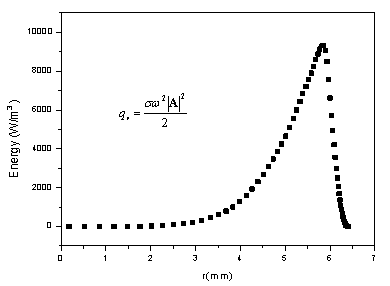
\includegraphics[width=0.95\textwidth]  {fig2.png}} 
\caption{内热源沿径向的分布}
\end{figure}

\begin{table}[!htbp]
\centering
\caption{高频感应加热的基本参数}
\begin{tabular}{|c| c|c|c|}
\hline
感应频率 &感应发生器功率 & 工件移动速度  &感应圈与零件间隙\\
(KHz)&($\% \times$80Kw) &(mm/min)  &(mm)\\
\hline
250 &88 &5900 &1.65\\
\hline
250 &88 &5900 &1.65\\
\hline
250 &88 &5900 &1.65\\
\hline
250 &88 &5900 &1.65\\
\hline
250 &88 &5900 &1.65\\
\hline
250 &88 &5900 &1.65\\
\hline
250 &88 &5900 &1.65\\
\hline
250 &88 &5900 &1.65\\
\hline
\end{tabular}
\end{table}

\begin{table}
\centering
\captionsetup{singlelinecheck=off}
\caption*{续表} %取消编号
\begin{tabular}{|c| c|c|c|}
\hline
感应频率 &感应发生器功率 & 工件移动速度  &感应圈与零件间隙\\
(KHz)&($\% \times$80Kw) &(mm/min)  &(mm)\\
\hline
250 &88 &5900 &1.65\\
\hline
250 &88 &5900 &1.65\\
\hline
\end{tabular}
\end{table}
%表格太大需要转页时,需要在续表上方注明“续表”,表头也应重复排出。


\subsection{公式格式}

\vspace{-10mm}
\begin{eqnarray}
\frac{1}{\mu} \nabla^2A - j \omega \sigma A -\nabla(\frac{1}{\mu}) \times(\nabla \times A)+J_0=0
\end{eqnarray}

\subsection{本章小结}
本章介绍了……

\newpage